\documentclass[12pt,a4paper]{article}
\usepackage{ucebnice}
\usepackage{polynom}

\title{Logaritmické funkce}
\author{Ondřej Škubala}
\date{\today}

\begin{document}

\maketitle
\newpage

\section{Logaritmické funkce}


\begin{quotebox}
{„Vynález logaritmů … tím, že zkrátil práci, zdvojnásobil život astronoma.“}
{Pierre-Simon Laplace (1799)}
\end{quotebox}


\begin{historicalbox}

Myšlenka logaritmů vznikla jako odpověď na dlouhodobou potřebu zjednodušit tehdejší mimořádně náročné výpočty, 
v nichž se neustále objevovalo opakované násobení, dělení či mocnění, 
a které byly zvláště v astronomii, navigaci a kartografii natolik zdlouhavé, 
že jejich provádění mohlo zabrat celé hodiny soustředěné práce; 
ačkoli starověké civilizace velmi dobře rozuměly postupnému násobení i mocninám, 
chyběl jim jednotný a skutečně obecný nástroj, který by dokázal převést násobení 
na pouhou aditivní operaci, čímž by zásadně urychlil veškeré numerické výpočty.  

První skutečný průlom přišel na počátku 17. století, 
kdy skotský matematik \textbf{John Napier (1550–1617)} představil svůj koncept logaritmů 
a ukázal, že každé násobení lze nahradit sčítáním příslušných logaritmických hodnot — 
což představovalo naprostou revoluci v rychlosti tehdejší vědy. 
Napierova práce byla natolik zásadní, že se logaritmy prakticky okamžitě rozšířily 
mezi astronomy, kteří tehdy sestavovali obrovské trigonometrické tabulky pro určování polohy hvězd a planet, 
a také mezi námořní navigátory, kteří potřebovali rychlé a přesné přepočty souřadnic, kurzů a vzdáleností.  

Krátce poté navázal anglický matematik \textbf{Henry Briggs (1561–1630)}, 
jenž představil logaritmy se základem~10 — tzv. \textit{logaritmy dekadické}. 
Ty se díky své jednoduché stavbě, snadné tabulkovatelnosti a návaznosti 
na tehdy používaný desítkový systém rychle rozšířily po celé Evropě 
a staly se na několik století základním nástrojem vědeckých výpočtů.  

Zvláštní a často opomíjenou kapitolou je epizoda spojená s \textbf{Galileem Galileim (1564–1642)}, 
který se o existenci „nových logaritmických metod“ doslechl zcela náhodou — 
pouze z vyprávění kolegů astronomů, kteří tvrdili, že jakýsi skotský učenec přišel na způsob, 
jak jednodušeji měřit vzdálenosti hvězd a provádět výpočty, 
aniž by Galileo kdy Napierovu knihu držel v ruce nebo znal její detaily. 
Galileo, fascinován pouhou \emph{zvěstí o existenci nového typu počítání}, 
dokázal z prázdné informace odvodit vlastní, na tehdejší dobu neuvěřitelně přesnou představu 
o tom, co logaritmy jsou a k čemu se používají. (Je mi líto toho kdo to čte a pokud tak činíš, dojdi si pro jedničku).
Jeho úvahy v přednáškách z let 1610–1612 ukazují, že na základě pouhého principu 
„násobení převedeného na sčítání“ dokázal rekonstruovat základní logaritmické chování — 
je to jeden z nejpůsobivějších příkladů čisté matematické intuice v dějinách vědy.  

Skutečnou matematickou podstatu logaritmů však v plné šíři objasnil až 
švýcarský matematik \textbf{Leonhard Euler (1707–1783)}, 
který během 18. století definoval přirozený logaritmus pomocí integrálu, 
propojil jej s exponenciální funkcí $e^x$ 
a ukotvil logaritmy jako fundamentální stavební kámen matematické analýzy. 
Euler tak logaritmus povýšil z pouhého výpočetního triku 
na hluboký teoretický objekt, který se objevuje v diferenciálních rovnicích, 
nekonečných řadách, fyzikálních modelech růstu, úbytku i v popisu mnoha přírodních zákonitostí.  

Ačkoliv moderní kalkulačky i počítače nahradily historické logaritmické tabulky 
a legendární logaritmická pravítka, význam logaritmů tím nikterak nezeslábl — 
naopak se ještě zvýšil, protože logaritmická měřítka a logaritmické funkce 
přesně popisují intenzitu zvuku v decibelech, sílu zemětřesení na Richterově škále, 
kyselost roztoků na pH škále, rozpad radioaktivních látek, růst populací, 
šíření epidemií či dokonce složitost algoritmů v informatice, 
kde logaritmus vyjadřuje, jak rychle dokážeme třídit a vyhledávat v datech.  

Logaritmus se tak stal univerzálním jazykem všude tam, 
kde se změny neodehrávají pouhým přičítáním, nýbrž násobením, 
a představuje jeden z nejvýznamnějších matematických konceptů, 
který propojuje čistou matematiku, přírodní vědy i moderní technologie.
\end{historicalbox}

\begin{quotebox}
{„Zkrátit pracnost a zvýšit snadnost výpočtů.“}
{John Napier, \textit{Mirifici Logarithmorum Canonis Descriptio (1614)}}
\end{quotebox}

\section{Úvod}

Exponenciální funkce nám popisovala situace, v nichž se hodnota v každém kroku násobí stále stejným číslem, 
takže i nepatrná změna exponentu mohla způsobit výrazný růst nebo naopak rychlý pokles. 
\important{Logaritmická funkce} představuje opak tohoto pohledu:
\textit{logaritmus převádí velikosti čísel na velikosti exponentů}, 
a tím dokáže zpřehlednit i velmi rozsáhlé hodnoty, které by jinak bylo obtížné přímo porovnávat.

\smallskip
Díky této vlastnosti se logaritmické funkce objevují všude tam, 
\textbf{kde hodnoty rostou nebo klesají tak rychle}, 
že je běžné lineární měřítko nestačí zachytit. 
Pokud se dvě veličiny liší třeba i desetitisíckrát, 
jejich logaritmy se obvykle liší jen o několik málo jednotek, 
což umožňuje přehledně sledovat trendy, porovnávat rozsahy
a analyzovat i takové procesy, v nichž rozdíly velikostí přesahují naše běžné intuitivní představy.

\smallskip
Zásadní roli hraje skutečnost, že logaritmus je \important{inverzní funkcí} k exponenciále. 
To znamená, že tyto dvě funkce se dokonale doplňují: 
exponenciála proměňuje malé změny exponentu ve výrazné změny výsledku, 
zatímco logaritmus tento proces obrací a z velkých čísel vytváří hodnoty snadno uchopitelné. 

\smallskip
Tato vlastnost tvoří základ pro logaritmické rovnice, nerovnice, 
i pro praktické modelování jevů, jejichž chování je popsáno rychlým růstem nebo úbytkem.

% Graf log a exp funkce
\begin{center}
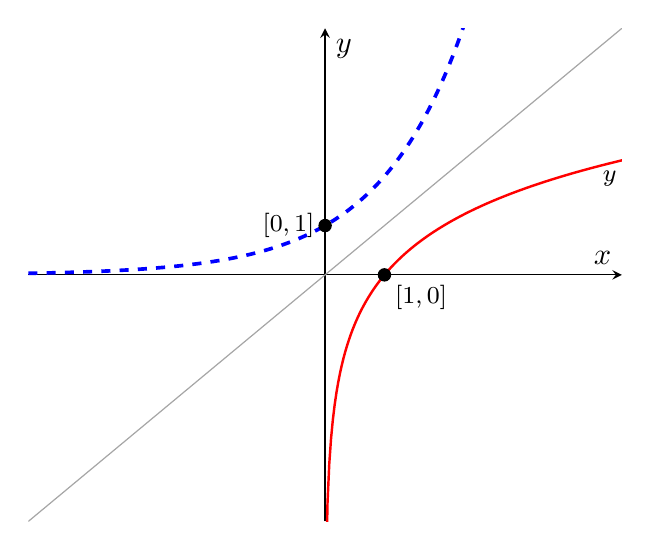
\begin{tikzpicture}[scale=1.1]
    \begin{axis}[
        axis lines=middle,
        xmin=-5, xmax=5,
        ymin=-5, ymax=5,
        xlabel={$x$},
        ylabel={$y$},
        ticks=none,
    ]

    % Přímka y = x
    \addplot[gray!70, thin] {x};

    % Exponenciála y = 2^x
    \addplot[blue, dashed, very thick, samples=200, domain=-5:6] {2^x};
    \node[above] at (axis cs: 3,5) {\footnotesize $y = 2^x$};

    % Logaritmus y = log_2 x
    \addplot[red, thick, samples=200, domain=0.01:6] {ln(x)/ln(2)};
    \node[right] at (axis cs:4.5,2) {\footnotesize $y = \log_2 x$};

    % Průsečík (1,0)
    \addplot[only marks, mark=*] coordinates {(1,0)};
    \node[below right] at (axis cs:1,0) {\footnotesize $[1,0]$};
    % Průsečík (0,1)
    \addplot[only marks, mark=*] coordinates {(0,1)};
    \node[left] at (axis cs:0,1) {\footnotesize $[0,1]$};
   
    \end{axis}
\end{tikzpicture}
\end{center}

Na obrázku je znázorněna \textbf{exponenciální funkce} $y = 2^x$ (čárkovaně), 
\textbf{logaritmická funkce} $y = \log_2 x$ (plnou čárou) a přímka $y = x$, 
podle níž jsou obě křivky vzájemně souměrné. 
Exponenciála prochází bodem $[0;1]$ a má vodorovnou asymptotu $y = 0$, 
zatímco logaritmus prochází bodem $[1;1]$ a má svislou asymptotu $x = 0$. 
Zatímco $2^x$ roste velmi rychle, $\log_2 x$ roste pomalu — 
každá funkce tak představuje inverzi té druhé.


% Graf log a exp funkce pro základ 1/2
\begin{center}
\begin{tikzpicture}[scale=1.1]
    \begin{axis}[
        axis lines=middle,
        xmin=-5, xmax=5,
        ymin=-3, ymax=5,
        xlabel={$x$},
        ylabel={$y$},
        ticks=none,
    ]

    % Přímka y = x
    \addplot[gray!70, thin] {x};

    % Exponenciála y = (1/2)^x
    \addplot[blue, dashed, very thick, samples=200, domain=-4:4.5] {(1/2)^x};
    \node[above] at (axis cs:-1.5,4) {\footnotesize $y = \left(\tfrac12\right)^x$};

    % Logaritmus y = log_{1/2} x
    \addplot[red, thick, samples=200, domain=0.05:4.5] {ln(x)/ln(1/2)};
    \node[right] at (axis cs:2.5,-1) {\footnotesize $y = \log_{\frac12} x$};

    % Průsečík (1,1)
    \addplot[only marks, mark=*] coordinates {(1,0)};
    \node[below right] at (axis cs:1,1) {\footnotesize $[1,0]$};

    % Exponenciála: průsečík (0,1)
    \addplot[only marks, mark=*] coordinates {(0,1)};
    \node[left] at (axis cs:0,1) {\footnotesize $[0,1]$};

    \end{axis}
\end{tikzpicture}
\end{center}

Na obrázku je znázorněna exponenciální funkce $y = \left(\tfrac12\right)^x$ (čárkovaně),
logaritmická funkce $y = \log_{\frac12} x$ (plnou čárou) a přímka $y = x$, 
která znázorňuje jejich inverzní vztah. 
Obě funkce jsou klesající: exponenciála se pro $x \to +\infty$ blíží k~nule, 
zatímco logaritmus se při přibližování k~nule zprava blíží k~-\(\infty\). 
Průsečíkem obou inverzních funkcí je bod $[1;1]$.



\subsection{Různé základy logaritmů}

Logaritmická funkce může mít libovolný základ $a$, který je kladný a zároveň různý od jedné, 
a právě volba tohoto základu \important{určuje rychlost růstu či poklesu celé funkce}. 
Pokud je základ \textbf{větší než jedna}, například $a = 2$ nebo $a = 10$, 
logaritmus je rostoucí funkcí, jejíž graf se zvedá pomalu, avšak nepřetržitě, 
a každé jeho zvýšení odpovídá násobnému zvětšení argumentu. 
Když je základ naopak \textbf{menší než jedna}, třeba $a = \tfrac12$, 
logaritmus se stává funkcí \textbf{klesající}, protože každé násobení takovým základem zmenšuje hodnotu výsledku, 
a logaritmus tak převádí velká čísla na menší a malá na větší v opačném pořadí než u rostoucích funkcí.

Výběr základu přitom není libovolný — každé užití má svůj typický kontext. 
Dekadický logaritmus $\log_{10} x$ se tradičně používá tam, kde se pracuje s \important{řády velikosti}, 
a proto se objevuje v chemii (pH), akustice (decibely) či v geofyzice (Richterova škála). 
Přirozený logaritmus $\ln x = \log_e x$ je \textbf{nejdůležitějším matematickým logaritmem}, 
neboť jeho základ $e$ má jedinečné vlastnosti v diferenciálním a integrálním počtu, 
v modelování růstu a v teorii pravděpodobnosti. 
Logaritmy se základem větším než jedna tedy sdílejí podobný tvar, 
liší se pouze \important{strmostí grafu}, 
zatímco logaritmy se základem mezi nulou a jedničkou jsou jejich zrcadlovým obrazem 
podle osy $y = x$ a mají klesající průběh.

Ve skutečnosti však nezáleží na tom, jaký kladný základ zvolíme, 
protože \textbf{všechny logaritmy se liší pouze konstantním násobkem}. 
Platí totiž \important{vzorec změny základu}
\[
\log_a x = \frac{\log_b x}{\log_b a},
\]
jenž ukazuje, že logaritmus v jednom základu lze snadno přepočítat na jakýkoli jiný. 
Tento vzorec patří mezi \textbf{čtyři základní logaritmické vzorce}, 
jež budeme dále pravidelně používat při řešení logaritmických rovnic a úprav výrazů.

Grafické znázornění různých logaritmů pak pěkně ukazuje, 
jak se mění sklon křivky podle volby základu, přičemž všechny procházejí společným bodem $[1;0]$ 
a mají stejnou svislou asymptotu $x = 0$.



\begin{center}
    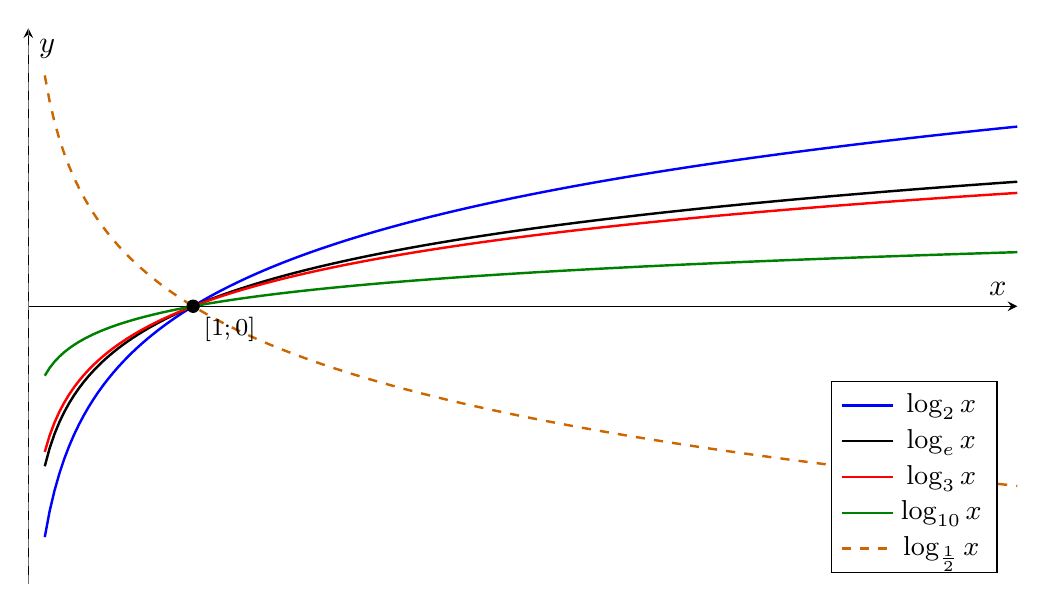
\begin{tikzpicture}[scale=1.1]
        \begin{axis}[
            axis lines=middle,
            xmin=0, xmax=6,
            ymin=-4, ymax=4,
            xlabel={$x$},
            ylabel={$y$},
            ticks=none,
            width=13cm,
            height=8cm,
            legend style={at={(0.98,0.02)}, anchor=south east, font=\small},
        ]
        
        % Logaritmus log_2 x
        \addplot[blue, thick, samples=200, domain=0.1:6] {ln(x)/ln(2)};
        \addlegendentry{$\log_2 x$}
        
        % Logaritmus log_2 x
        \addplot[black, thick, samples=200, domain=0.1:6] {ln(x)/ln(e)};
        \addlegendentry{$\log_e x$}
        
        % Logaritmus log_3 x
        \addplot[red, thick, samples=200, domain=0.1:6] {ln(x)/ln(3)};
        \addlegendentry{$\log_3 x$}
        
        % Logaritmus log_10 x
        \addplot[green!50!black, thick, samples=200, domain=0.1:6] {ln(x)/ln(10)};
        \addlegendentry{$\log_{10} x$}
        
        % Logaritmus log_(1/2) x
        \addplot[orange!80!black, dashed, thick, samples=200, domain=0.1:6] {ln(x)/ln(1/2)};
        \addlegendentry{$\log_{\frac12} x$}
        
        % Bod (1,0)
        \addplot[only marks, mark=*] coordinates {(1,0)};
        \node[below right] at (axis cs:1,0) {\footnotesize $[1;0]$};
        
        % Asymptota x=0
        \draw[dashed, gray!60] (axis cs:0,-4) -- (axis cs:0,4);
        \node[left] at (axis cs:0,3.5) {\footnotesize $x=0$};
        
        \end{axis}
    \end{tikzpicture}
\end{center}

\subsubsection*{Binární logaritmus — $\log_2 x$}
Binární logaritmus je logaritmus o základu $2$ a hraje klíčovou roli zejména v informatice, 
neboť \important{přirozeně popisuje procesy založené na zdvojnásobování nebo půlení}. 
Objevuje se ve složitosti algoritmů, ve vyhledávacích strukturách (např.~binární stromy) 
a v růstu objemu dat. 
Funkce $\log_2 x$ roste rychleji než dekadický logaritmus, 
což odráží skutečnost, že přechod mezi jednotlivými hodnotami odpovídá násobení dvěma, 
tedy základní operaci binárního systému.

\subsubsection*{Přirozený logaritmus — $\ln x$}
Přirozený logaritmus $\ln x$ je \textbf{nejdůležitějším logaritmem v matematické analýze}, 
protože jeho základ $e$ se přirozeně vyskytuje ve všech procesech spojitého růstu. 
Má jedinečnou vlastnost, že je to \important{jediný logaritmus, jehož derivace má jednoduchý tvar} 
$\frac{1}{x}$, což jej činí zásadním nástrojem v diferenciálním a integrálním počtu. 
Přirozený logaritmus se objevuje v modelech růstu a úbytku, v teorii pravděpodobnosti, 
ve fyzice, ekonomii i statistice, a proto jej lze považovat 
za „standardní“ logaritmus v mnoha matematických disciplínách.

\subsubsection*{Dekadický logaritmus — $\log_{10} x$}
Dekadický logaritmus, označovaný jako $\log_{10} x$, se používá tam, 
kde \important{pracujeme s řády velikosti}, protože základ $10$ odpovídá 
našemu desetinnému systému. 
Objevuje se v mnoha praktických měřítkách: v chemii (pH), v akustice (decibely), 
v geologii (Richterova škála), ale také v technických disciplínách a inženýrských výpočtech. 
Graf $\log_{10} x$ roste pomaleji než $\log_2 x$, 
což odpovídá tomu, že k posunu o jednu jednotku logaritmu je třeba zvětšit argument desetkrát.

\subsubsection*{Logaritmus se základem $\tfrac12$ — $\log_{\frac12} x$}
Logaritmus o základu menším než jedna je \textbf{klesající funkcí}, 
což je výrazný rozdíl oproti běžným logaritmům se základem větším než jedna. 
Funkce $\log_{\frac12} x$ \important{převrací pořadí hodnot}: 
čím je argument větší, tím menší je hodnota logaritmu. 
Tento logaritmus je často uváděn jako ukázkový příklad inverzního chování logaritmu, 
jenž doplňuje rostoucí logaritmy a přehledně ilustruje závislost průběhu funkce na volbě základu.


\begin{examplebox}
    
    \textbf{Základní logaritmická funkce $y = \log_2 x$}

    Základní funkce $y = \log_2 x$ je rostoucí funkce se svislou asymptotou $x = 0$. 
    Prochází bodem $[1;0]$ a její graf se zvedá stále pomaleji, 
    což je typický tvar všech rostoucích logaritmů.

    \begin{center}
        \begin{tikzpicture}[scale=1.0]
            \begin{axis}[
                axis lines=middle,
                xmin=-1, xmax=6,
                ymin=-3, ymax=3,
                ticks=none,
                width=10cm,
                height=7cm
            ]
            
            % log_2 x
            \addplot[blue, thick, samples=200, domain=0.1:6] {ln(x)/ln(2)};
            \node[right] at (axis cs:5,1.3) {\footnotesize $y = \log_2 x$};
            
            % asymptota
            \draw[dashed, gray!70] (axis cs:0,-3) -- (axis cs:0,3);
            
            \end{axis}
        \end{tikzpicture}
    \end{center}

    Výraz $(x - 2)$ uvnitř logaritmu znamená \textbf{posun celého grafu o 2 jednotky doprava}. 
    Tvar grafu zůstává stejný, pouze se změní jeho poloha. 
    Asymptota se přesouvá z $x = 0$ na $x = 2$.

    \begin{center}
        \begin{tikzpicture}[scale=1.0]
            \begin{axis}[
                axis lines=middle,
                xmin=-1, xmax=8,
                ymin=-3, ymax=3,
                ticks=none,
                width=10cm,
                height=7cm
            ]
            
            % původní logaritmus (světle)
            \addplot[blue!30, thick, samples=200, domain=0.1:6] {ln(x)/ln(2)};
            
            % nový logaritmus
            \addplot[red, thick, samples=200, domain=2.1:8] {ln(x-2)/ln(2)};
            \node[right] at (axis cs:5,1.2) {\footnotesize $y = \log_2(x-2)$};
            
            % asymptota po posunu
            \draw[dashed, gray!70] (axis cs:2,-3) -- (axis cs:2,3);
            \node[above left] at (axis cs:2,2) {\footnotesize $x = 2$};
            
            \end{axis}
        \end{tikzpicture}
    \end{center}

    Přičtení konstanty $+3$ způsobí \textbf{posun celého grafu o 3 jednotky nahoru}. 
    Asymptota i tvar funkce zůstávají stejné, mění se pouze výška grafu.

    \begin{center}
        \begin{tikzpicture}[scale=1.0]
            \begin{axis}[
                axis lines=middle,
                xmin=-1, xmax=8,
                ymin=-3, ymax=6,
                ticks=none,
                width=10cm,
                height=7cm
            ]
            
            % předchozí graf (log_2(x-2))
            \addplot[red!30, thick, samples=200, domain=2.1:8] {ln(x-2)/ln(2)};
            
            % nový graf
            \addplot[purple, thick, samples=200, domain=2.1:8] {ln(x-2)/ln(2) + 3};
            \node[right] at (axis cs:4,5.5) {\footnotesize $y = \log_2(x-2) + 3$};
            
            % asymptota zůstává na x = 2
            \draw[dashed, gray!70] (axis cs:2,-3) -- (axis cs:2,6);
            \node[above left] at (axis cs:2,5) {\footnotesize $x = 2$};
            
            \end{axis}
        \end{tikzpicture}
    \end{center}

\end{examplebox}


\begin{notebox}
\textbf{Asymptota} je přímka, ke které se graf funkce stále přibližuje, 
ale nikdy jí nedosáhne.  
U logaritmických funkcí je důležitá zejména \important{svislá asymptota} — 
např. u $y = \log_2 x$ je to přímka \textbf{$x = 0$}. 
Po posunu funkce se asymptota posune spolu s ní (např. $x = 2$ u $y = \log_2(x-2)$).
\end{notebox}



% -----------------------------------------------------------------
% ---------------------- P Ř Í K L A D Y --------------------------
% -----------------------------------------------------------------

\exercisepart
\setcounter{section}{1}

% =========================
% ÚLOHA 1 – Grafy logaritmických funkcí
% =========================
\begin{exercise}[Načrtněte grafy logaritmických funkcí]
    Načrtněte grafy následujících logaritmických funkcí:
    \begin{tasks}(2)
        \task $y = \log_3 x$
        \task $y = \log_{\frac13} x$
        \task $y = \log_4 x$
        \task $y = \log_{\frac14} x$
        \task $y = \log_{10} x$
        \task $y = \log_{\frac1{10}} x$
        \task $y = \log_2 x$
        \task $y = \log_{\frac12} x$
        \task $y = \ln x$
        \task $y = \log_{\frac1e} x$
    \end{tasks}
\end{exercise}


% =========================
% ÚLOHA 2 – Rozhodněte, které výrazy jsou kladné
% =========================
\begin{exercise}[Rozhodněte, které z následujících výrazů jsou kladné]
    Rozhodněte, které z následujících čísel jsou kladné:
    \begin{tasks}(2)
        \task $\log_{0.5} 6$
        \task $\log_{14} (-11)$
        \task $-\log_{0.6} 15$
        \task $\log_7 8$
        \task $-\ln 1$
        \task $\log_{\frac12} (-6)$
        \task $\log_3 0.4$
        \task $\log_{\frac14} 10$
        \task $-\log_{9} \dfrac{1}{3}$
        \task $\ln (e^5)$
        \task $\log_5 1.2$
        \task $-\log_{2} 0.25$
    \end{tasks}
\end{exercise}


% =========================
% ÚLOHA 3 – Definiční obory
% =========================
\begin{exercise}[Zjistěte definiční obory následujících funkcí]
    Zjistěte definiční obory následujících funkcí:
    \begin{tasks}(2)
        \task $y = \log_{10}(x + 3)$
        \task $y = \log_2(-x)$
        \task $y = \ln\left(\sqrt{5 - x}\right)$
        \task $y = \sqrt{\log_3(x)}$
        \task $y = \log_{\frac12}(4 - 2x)$
        \task $y = \ln(x^2 - 9)$
        \task $y = \log_7\left(\dfrac{x}{x - 1}\right)$
        \task $y = \sqrt{-\ln(x)}$
        \task $y = \log_5(x^2 + x - 6)$
        \task $y = \dfrac{1}{\log_4(x - 2)}$
    \end{tasks}
\end{exercise}


% =========================
% ÚLOHA 4 – Logaritmické nerovnice (monotónnost)
% =========================
\begin{exercise}[Najděte všechna $x \in \mathbb{R}$, pro která platí]
    Najděte všechna $x \in \mathbb{R}$, pro která platí:
    \begin{tasks}(2)
        \task $\log_2(x) > \log_2(4)$
        \task $\log_{0.5}(x) \ge \log_{0.5}(2)$
        \task $\log_x(3) < \log_x(11)$
        \task $\log_3(x - 1) \le \log_3(8)$
        \task $\log_{0.5}(2x + 1) < \log_{0.5}(5)$
        \task $\ln(x - 1) < \ln(5)$
        \task $\log_7(2x + 1) \ge \log_7(15)$
        \task $\log_{0.2}(3 - x) < \log_{0.2}(1)$
        \task $\log_x(5) > 1$
        \task $\log_3(x^2 - 4) \ge \log_3(5)$
    \end{tasks}
\end{exercise}

\setcounter{section}{2}
% =========================
% ÚLOHA 5 – Exponenciální růst v biologii
% =========================
\begin{exercise}[Růst bakteriální kultury]
    Počet bakterií jisté kultury vzroste za jednu hodinu o \(32\,\%\).  
    Vyjádřete závislost počtu bakterií na čase:
    \begin{tasks}(1)
        \task pomocí vzorce \(N_t = N_0 \cdot a^t\),
        \task pomocí vzorce \(N_t = N_0 \cdot e^{\lambda t}\),
    \end{tasks}
    kde \(N_0\) je počáteční počet bakterií, \(t\) je čas v hodinách,  
    \(a\) je růstový faktor a \(\lambda\) je růstová konstanta.
\end{exercise}


% =========================
% ÚLOHA 6 – Newtonův zákon ochlazování
% =========================
\begin{exercise}[Ochlazování vody]
    Voda v nádobě má počáteční teplotu \(t_1 = 80\,^\circ\mathrm{C}\), 
    okolní prostředí má teplotu \(t_2 = 15\,^\circ\mathrm{C}\).  
    Závislost teploty vody na čase \(\tau\) (v minutách) je dána přibližným vztahem
    \[
    t = t_2 + (t_1 - t_2)\, e^{-0.05\tau}.
    \]
    Vypočítejte teplotu vody:
    \begin{tasks}(1)
        \task po \(5\) minutách,
        \task po \(60\) minutách.
    \end{tasks}
\end{exercise}


% =========================
% ÚLOHA 7 – Richterova škála
% =========================
\begin{exercise}[Zemětřesení – Richterova škála]
    Magnituda zemětřesení na Richterově škále je dána vztahem
    \[
    M = \log_{10}\!\left(\frac{I}{I_0}\right),
    \]
    kde \(I\) je intenzita zemětřesení a \(I_0\) je referenční intenzita.
    Určete:
    \begin{tasks}(1)
        \task o kolik je silnější zemětřesení o magnitudě \(M = 6{,}2\) oproti zemětřesení o magnitudě \(M = 4{,}2\);
        \task kolikrát je intenzita zemětřesení o magnitudě \(M = 5\) větší než intenzita o magnitudě \(M = 3\).
    \end{tasks}
\end{exercise}


% =========================
% ÚLOHA 8 – Chemie: pH roztoku
% =========================
\begin{exercise}[Výpočet pH roztoku]
    pH je definováno vztahem
    \[
    \mathrm{pH} = -\log_{10}[H^+],
    \]
    kde \([H^+]\) je koncentrace vodíkových iontů v mol/l.
    Vypočítejte:
    \begin{tasks}(1)
        \task pH roztoku s koncentrací \([H^+] = 3 \cdot 10^{-4}\,\text{mol/l}\);
        \task koncentraci \([H^+]\) roztoku, jehož pH je \(2{,}8\).
    \end{tasks}
\end{exercise}


% =========================
% ÚLOHA 9 – Akustika: intenzita zvuku
% =========================
\begin{exercise}[Hladina intenzity zvuku]
    Hladina intenzity zvuku v decibelech je dána vzorcem
    \[
    L = 10 \log_{10}\!\left(\frac{I}{I_0}\right),
    \]
    kde \(I\) je intenzita zvuku a \(I_0\) je referenční intenzita.
    Určete:
    \begin{tasks}(1)
        \task o kolik dB je hlasitější zvuk o intenzitě \(I = 1000\, I_0\);
        \task kolikrát je intenzita zvuku vyšší, pokud hladina vzroste o \(20\,\mathrm{dB}\).
    \end{tasks}
\end{exercise}


% =========================
% ÚLOHA 10 – Astronomie: magnituda hvězd
% =========================
\begin{exercise}[Jasnost hvězd – astronomická magnituda]
    Rozdíl magnitud dvou hvězd je definován vztahem
    \[
    m_1 - m_2 = -2.5 \log_{10}\!\left(\frac{F_1}{F_2}\right),
    \]
    kde \(F_1\) a \(F_2\) jsou jejich světelné toky (jasnosti).
    Určete:
    \begin{tasks}(1)
        \task kolikrát je jasnější hvězda o magnitudě \(m = 1\) než hvězda o magnitudě \(m = 6\);
        \task jaká je magnituda hvězdy, jejíž jasnost je \(100\)-krát větší než jasnost hvězdy s magnitudou \(m = 5\).
    \end{tasks}
\end{exercise}



\end{document}

